% ---------------------------------------------------------------- 39
% [suite]
\begin{frame}{Ce qu'une p-value dit — et ne dit pas}
\begin{columns}[t]
\begin{column}{0.48\textwidth}
\begin{solbox}[Ce qu'elle dit]
$p = P\big(T \text{ aussi extrême} \given H_0 \text{ vraie}\big)$

\vspace{1mm}
C'est une probabilité \textbf{des données}, conditionnelle à une hypothèse
que l'on n'a jamais testée directement. C'est une mesure de
\emph{surprise}, pas une mesure de \emph{preuve}.
\end{solbox}
\end{column}
\begin{column}{0.48\textwidth}
\begin{kbox}[La traduction bayésienne]
\[
\underbrace{\frac{P(H_0 \given y)}{P(H_1 \given y)}}_{\text{ce qui intéresse}}
=
\underbrace{\frac{P(H_0)}{P(H_1)}}_{\text{le contexte}}
\times
\underbrace{BF_{01}}_{\text{l'évidence}}
\]
Le bayésien rend explicites les deux facteurs que la p-value
\textbf{mélange} et cache.
\end{kbox}
\begin{ebox}[Chiffre à retenir de la simulation]
Sur 3 000 tests simulés avec $H_0$ \emph{réellement vraie}, la distribution
des p-values est \textbf{uniforme} : 5 \% des études afficheront $p < 0{,}05$
par pur hasard. Le seuil n'est pas une garantie.
\end{ebox}
\end{column}
\end{columns}
\end{frame}

% [suite]
\begin{frame}{Ce qu'une p-value dit — et ne dit pas (suite)}
\begin{wbox}[Ce qu'elle ne dit pas]
\begin{itemize}
  \item \nok{} $p = 0{,}03$ ne signifie pas « 3 \% de chance que $H_0$ soit vraie ».
  \item \nok{} $p > 0{,}05$ ne signifie pas « pas d'effet » : c'est
        « pas assez de données pour trancher ».
  \item \nok{} $p$ n'a pas d'interprétation \emph{après} avoir vu les données
        comme probabilité d'hypothèse.
  \item \nok{} $p$ dépend de l'intention d'arrêter l'expérience (arrêt séquentiel,
        tests multiples).
\end{itemize}
\end{wbox}
\end{frame}

% ---------------------------------------------------------------- 40
\begin{frame}{Sept avantages concrets du bayésien}
\begin{columns}[t]
\begin{column}{0.49\textwidth}
\begin{enumerate}
  \item \textbf{Réponse directe.} « $P(\theta > 0{,}5 \given y) = 0{,}975$ » :
        la question du décideur, sans traduction.
  \item \textbf{Information externe incorporée} explicitement et de façon
        auditable (prior, power prior, méta-analyse).
  \item \textbf{Petits échantillons maîtrisés} : le prior régularise
        (\emph{shrinkage}) au lieu de laisser exploser la variance.
  \item \textbf{Arrêt séquentiel licite} : la conclusion est conditionnelle aux
        données observées — un essai peut s'arrêter dès que la preuve est suffisante.
\end{enumerate}
\end{column}
\begin{column}{0.49\textwidth}
\begin{enumerate}
  \setcounter{enumi}{4}
  \item \textbf{Modèles hiérarchiques naturels} : les groupes échangent
        de l'information, indispensable pour les données groupées.
  \item \textbf{Propagation complète de l'incertitude} : la prédiction intègre
        l'incertitude des paramètres, des effets latents et du bruit.
  \item \textbf{Mise à jour continue} : le posterior d'aujourd'hui est le prior
        de demain, idéal pour un système en production.
\end{enumerate}
\vspace{1mm}
\begin{kbox}[Contrepartie honnête]
Aucun de ces avantages n'est gratuit : le prior doit être
\textbf{choisi, écrit et défendu}.
\end{kbox}
\end{column}
\end{columns}
\end{frame}

% ---------------------------------------------------------------- 41
\begin{frame}{Limites, coûts et objections légitimes}
\begin{columns}[t]
\begin{column}{0.48\textwidth}
\begin{wbox}[Les cinq coûts réels]
\begin{enumerate}
  \item \textbf{Calcul} : intégrales sans forme close $\Rightarrow$ MCMC.
        Notre régression à 3 paramètres : 160 s sur CPU ; un modèle hiérarchique
        réel demande des heures et un GPU.
  \item \textbf{Choix du prior} : impossible à automatiser, doit être justifié.
        Un prior vague n'est pas neutre, il est souvent pire qu'un prior réfléchi.
  \item \textbf{Diagnostic} : une chaîne qui n'a pas convergé produit des nombres
        \emph{faux mais crédibles}. Il faut apprendre à lire $\hat R$, ESS, trace.
  \item \textbf{Robustesse} : un prior mal calibré donne une réponse
        précise et erronée (slide 36).
  \item \textbf{Culture} : beaucoup de collègues, de revues et de jurys
        raisonnent encore en p-values.
\end{enumerate}
\end{wbox}
\end{column}
\begin{column}{0.48\textwidth}
\begin{kbox}[Objections fréquentes, réponses]
\textbf{« Le prior rend le résultat subjectif. »} \\
Tout modèle contient des choix subjectifs ; le bayésien est le seul à les
\emph{écrire}. Le test fréquentiste cache ses choix dans le plan d'analyse.

\vspace{1.5mm}
\textbf{« Avec beaucoup de données, le prior n'importe plus. »} \\
Vrai asymptotiquement (les données dominent en $n$), faux en pratique :
avec des données groupées ou peu nombreuses, le prior décide.

\vspace{1.5mm}
\textbf{« C'est trop lent pour la production. »} \\
Faux : la phase coûteuse est \emph{hors ligne} ; la prédiction en ligne
se fait par $\theta$ échantillonné, en microsecondes.
\end{kbox}
\end{column}
\end{columns}
\end{frame}

% ---------------------------------------------------------------- 42
\begin{frame}{Le détour par le fréquentiste : planifier une étude}
\begin{center}
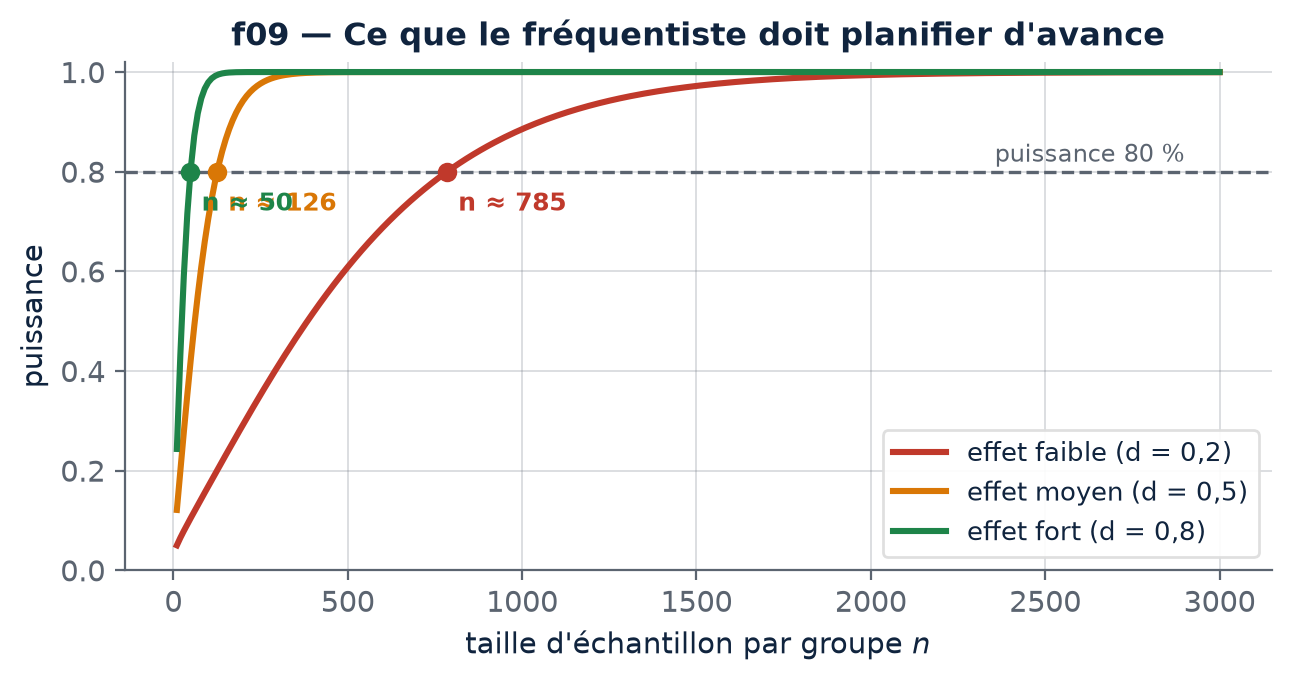
\includegraphics[width=0.58\textwidth]{f09_puissance.png}
\end{center}
\vspace{-1mm}
\begin{columns}[t]
\begin{column}{0.6\textwidth}
\begin{tabular}{@{}lccc@{}}
\toprule
Taille d'effet & $d = 0{,}2$ (faible) & $d = 0{,}5$ (moyen) & $d = 0{,}8$ (fort) \\
\midrule
$n$ par groupe pour 80 \% de puissance & 785 & 126 & 50 \\
\bottomrule
\end{tabular}
\vspace{1mm}

\small Calculé par la formule usuelle $n = 4(z_{1-\alpha/2}+z_{\text{puiss.}})^2/d^2$
(script \file{src/fig\_ch1.py}).
\end{column}
\begin{column}{0.38\textwidth}
\begin{kbox}[La réponse bayésienne]
Au lieu de fixer $n$ à l'avance, on suit
$P(\theta > \text{seuil} \given y_{1..n})$ et on arrête quand elle dépasse
un niveau fixé \textbf{avant} l'étude : la logique des essais adaptatifs.
\end{kbox}
\end{column}
\end{columns}
\end{frame}

% ---------------------------------------------------------------- 43
\begin{frame}{L'écosystème logiciel : quoi utiliser, quand}
% [rogna]
\footnotesize
\begin{center}
\footnotesize
{\setlength{\tabcolsep}{3pt}\begin{tabular}{@{}p{1.9cm}p{2.3cm}p{2.1cm}p{2.8cm}p{2.4cm}@{}}
\toprule
\textbf{Outil} & \textbf{Langage} & \textbf{Échantillonneur} & \textbf{Points forts} & \textbf{Quand le choisir} \\
\midrule
\textbf{PyMC} & Python & NUTS (PyTensor) & intégration NumPy/Pandas, ArviZ,
modèles hiérarchiques & \textbf{notre choix dans ce cours} \\
\textbf{Stan} & C++ $+$ R/Python & NUTS & référence en performance,
écosystème académique & modèles lourds, publication \\
\textbf{JAGS} & R & Gibbs & historique, très lisible & enseignement, modèles simples \\
\textbf{NumPyro} & Python & NUTS (JAX) & rapide, vectorisé, GPU & grands modèles, production \\
\textbf{ArviZ} & Python & --- & diagnostics et visualisation & avec PyMC ou NumPyro \\
\textbf{R} ($+$ \texttt{bayesplot}) & R & --- & graphiques prêts pour publication &
public cible R \\
\textbf{INLA} & R & Laplace déterministe & très rapide (GMRF) & champs gaussiens \\
\bottomrule
\end{tabular}}
\end{center}
\vspace{1mm}
\begin{kbox}[Le conseil du cours]
Un seul écosystème suffit pour tout apprendre : \textbf{Python $+$ PyMC $+$ ArviZ}.
Tout ce qui suit est exécutable sur un ordinateur portable sans GPU.
\end{kbox}
\end{frame}

% ---------------------------------------------------------------- 44
\begin{frame}[fragile]{Premier modèle complet — à taper et exécuter}
\begin{columns}[t]
\begin{column}{0.53\textwidth}
\begin{codebox}[premier\_modele.py]
\begin{lstlisting}
import pymc as pm
import arviz as az
import numpy as np

n, k = 10, 7

with pm.Model() as modele:
    theta = pm.Beta("theta", alpha=2, beta=2)      # prior
    pm.Binomial("y", n=n, p=theta, observed=k)     # vraisemblance

    # 1. echantillonnage a posteriori
    trace = pm.sample(draws=2000, tune=1000, chains=2)

    # 2. prediction pour 5 nouveaux lancers
    y_new = pm.Binomial("y_new", n=5, p=theta,
                        shape=5, observed=None)
    pred = pm.sample_posterior_predictive(trace)

print(az.summary(trace, hdi_prob=0.95))
print(pred.posterior_predictive["y_new"].mean())
\end{lstlisting}
\end{codebox}
\end{column}
\begin{column}{0.45\textwidth}
\begin{abox}[Lancez-le maintenant]
\begin{itemize}
  \item Sur cette machine (CPU, 2 chaînes, 3 000 itérations) :
        \textbf{5,8 secondes}.
  \item Vous venez d'estimer une distribution a posteriori complète
        sans écrire une seule intégrale.
\end{itemize}
\end{abox}
\begin{kbox}[Sortie attendue]
\begin{tabular}{@{}ll@{}}
postérieur moyen & $0{,}648$ \\
écart-type & $0{,}124$ \\
crédibilité 95 \% & $[0{,}383 \,;\, 0{,}864]$ \\
$\hat R$ & $1{,}0005$ \\
ESS & $1\,514$ \\
\end{tabular}
\vspace{1mm}

\footnotesize $1\,514$ tirages indépendants équivalents sur $4\,000$ : la chaîne
a une mémoire modérée, c'est acceptable.
\end{kbox}
\end{column}
\end{columns}
\end{frame}

% ---------------------------------------------------------------- 45
% [rogna]
% [rogna]
% [rogna]
\begin{frame}{Lire un résultat PyMC sans se tromper}
\begin{center}
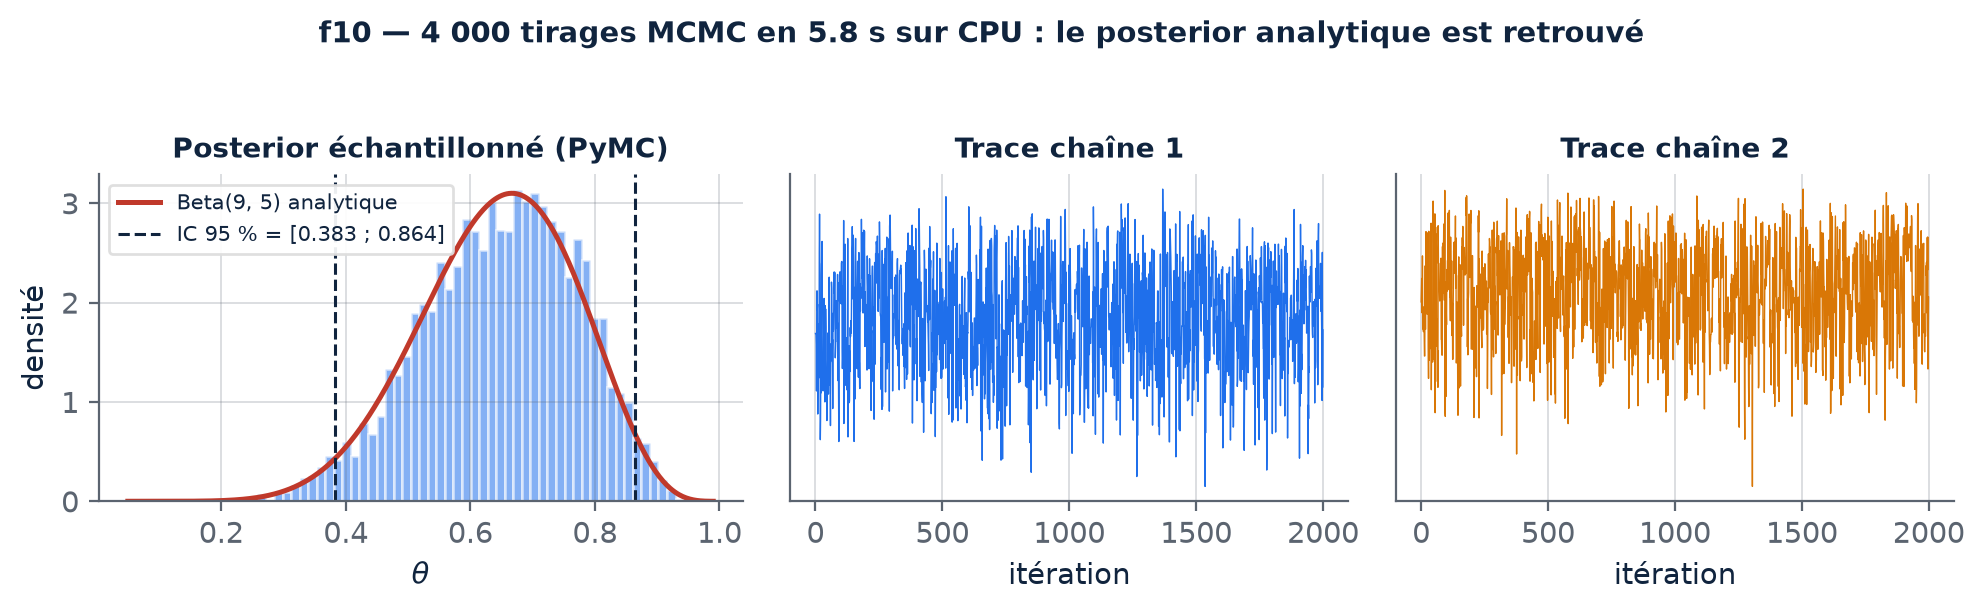
\includegraphics[width=.78\textwidth]{f10_pymc_coin.png}
\end{center}
\vspace{-1.5mm}
\begin{center}
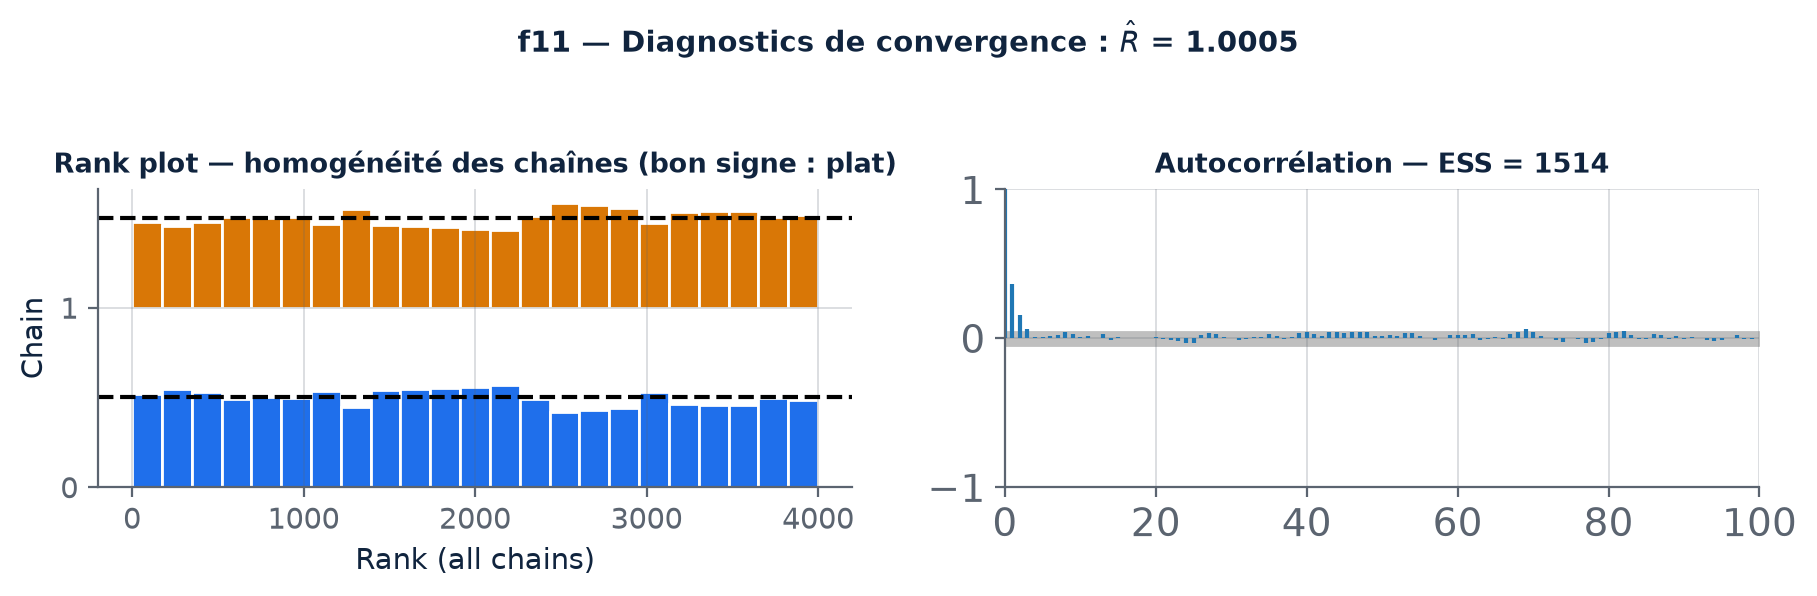
\includegraphics[width=.58\textwidth]{f11_pymc_diagnostics.png}
\end{center}
\vspace{-1mm}
\centering\small
L'histogramme des tirages MCMC reproduit la densité analytique $\mathrm{Beta}(9,5)$ (trait rouge) :
l'échantillonneur ne « fabrique » pas une réponse, il explore une densité.
Le \emph{rank plot} plat et l'autocorrélation qui retombe en quelques dizaines
d'itérations sont les deux signes d'une chaîne saine.
\end{frame}

% ---------------------------------------------------------------- 46
% [suite]
\begin{frame}{Les huit pièges du débutant}
\begin{columns}[t]
\begin{column}{0.48\textwidth}
\begin{wbox}[Pièges de modélisation]
\begin{enumerate}
  \item \textbf{Confondre prior et posterior} : le prior est avant les données,
        et il ne doit jamais être présenté comme un résultat.
  \item \textbf{Prior trop informatif sans justification} : c'est le prior qui
        décide, pas les données (slide 36).
  \item \textbf{Prior vague pris pour neutre} : sur une échelle
        ($\log\sigma$, une variance, une probabilité), le prior uniforme
        \emph{n'est pas} neutre.
  \item \textbf{Oublier la prédiction} : un modèle qui n'est jamais confronté
        à de nouvelles données n'est pas validé.
\end{enumerate}
\end{wbox}
\end{column}
\begin{column}{0.48\textwidth}
\begin{wbox}[Pièges de calcul et de lecture]
\begin{enumerate}
  \setcounter{enumi}{4}
  \item \textbf{Ignorer les diagnostics} : $\hat R > 1{,}01$ ou ESS faible
        invalident tout le reste.
  \item \textbf{Ne publier que la moyenne} : l'incertitude \emph{est} le résultat.
  \item \textbf{Interpréter le crédible comme un IC} : ce sont deux objets
        mathématiques distincts (slide 37).
  \item \textbf{Traiter le posterior d'un modèle A comme le prior d'un modèle B} :
        changer de modèle invalide le posterior.
\end{enumerate}
\end{wbox}
\end{column}
\end{columns}
\vspace{1mm}
\end{frame}

% [suite]
\begin{frame}{Les huit pièges du débutant (suite)}
\begin{kbox}[La question qui sauve]
Pour chaque affirmation numérique : \textbf{« est-elle robuste à un changement
raisonnable de prior ? »} Si non, elle ne vaut rien.
\end{kbox}
\end{frame}

% ---------------------------------------------------------------- 47
\begin{frame}{Checklist de l'analyse bayésienne}
\begin{columns}[t]
\begin{column}{0.50\textwidth}
\begin{abox}[Avant de lancer l'échantillonnage]
\begin{enumerate}
  \item Le modèle est-il écrit ? (vraisemblance $+$ priors, explicitement)
  \item Chaque prior a-t-il une \textbf{unité} et une \textbf{échelle} raisonnables ?
  \item Les variables sont-elles \textbf{centrées et réduites} ?
  \item Un \textbf{prior predictive check} a-t-il été fait ?
  \item Le modèle génère-t-il des données qui ressemblent au réel ?
\end{enumerate}
\end{abox}
\end{column}
\begin{column}{0.48\textwidth}
\begin{solbox}[Après l'échantillonnage]
\begin{enumerate}
  \item $\hat R < 1{,}01$ pour \textbf{tous} les paramètres ?
  \item ESS $> 400$ (idéalement 1 000) par paramètre ?
  \item Trace plot : pas de dérive, pas de \emph{sticky} ?
  \item Divergences : zéro (sinon reparamétrer) ?
  \item \textbf{Posterior predictive check} : le modèle reproduit-il les données ?
  \item Sensibilité au prior : les conclusions tiennent-elles ?
\end{enumerate}
\end{solbox}
\end{column}
\end{columns}
\vspace{1.5mm}
\begin{kbox}[Livrable minimal d'une analyse bayésienne]
Modèle, priors justifiés, diagnostics, posterior, prédiction, sensibilité.
\end{kbox}
\end{frame}

% ---------------------------------------------------------------- 48
\begin{frame}{Quiz de synthèse du chapitre 1}
\begin{qbox}[Cinq questions — 6 minutes, puis correction]
\begin{enumerate}
  \item Un test a une sensibilité de 99 \% et une spécificité de 95 \%.
        La prévalence est 1 \%. Un patient est positif.
        La probabilité qu'il soit malade vaut \dots
        (A) 95 \% \quad (B) 66 \% \quad (C) 17 \% \quad (D) 5 \%
  \item Un intervalle de crédibilité à 95 \% signifie \dots
        (A) 95 \% des échantillons donneraient cet intervalle \quad
        (B) 95 \% de chance que $\theta$ y soit \quad
        (C) 95 \% des données y sont
  \item Après un prior $\mathrm{Beta}(1,1)$ et 7 succès sur 10, la moyenne
        a posteriori vaut \dots
        (A) 0,700 \quad (B) 0,667 \quad (C) 0,643 \quad (D) 0,500
  \item Une p-value de 0,05 avec un prior neutre laisse
        $P(H_0 \given y)$ proche de \dots
        (A) 0,05 \quad (B) 0,50 \quad (C) 0,71 \quad (D) 0,95
  \item Le posterior d'un modèle peut servir de prior \dots
        (A) toujours \quad (B) pour de nouvelles données du \emph{même} modèle
        \quad (C) jamais
\end{enumerate}
\end{qbox}
\end{frame}

% ---------------------------------------------------------------- 49
\begin{frame}{Correction et barème}
\begin{columns}[t]
\begin{column}{0.55\textwidth}
\begin{solbox}[Réponses]
\begin{enumerate}
  \item \textbf{(C) 17 \%} — $0{,}99\times0{,}01 / (0{,}0099+0{,}0495) = 0{,}167$.
        Le nombre de faux positifs écrase le nombre de vrais positifs.
  \item \textbf{(B)} — c'est une probabilité \emph{sur le paramètre}, conditionnelle
        aux données et au prior.
  \item \textbf{(B) 0,667} — $\mathrm{Beta}(8,4)$, moyenne $8/12$.
        La réponse (C) correspond au prior $\mathrm{Beta}(2,2)$.
  \item \textbf{(C) 0,71} — $BF_{01} = 2{,}46$ avec un prior neutre.
  \item \textbf{(B)} — uniquement pour des données du même modèle,
        avec la même vraisemblance.
\end{enumerate}
\end{solbox}
\end{column}
\begin{column}{0.43\textwidth}
\begin{abox}[Questions ouvertes]
\begin{itemize}
  \item Citez une étude de votre domaine où le prior aurait changé la conclusion.
        Quelle aurait été la source du prior ?
  \item Pourquoi le nombre de faux positifs croît-il quand la maladie devient rare ?
        Exprimez la condition sur la spécificité.
\end{itemize}
\end{abox}
\begin{kbox}[Indice pour la question 2]
$P(T^+ \given \bar M) < \dfrac{\text{prévalence}}{1-\text{prévalence}} \times \text{sensibilité}$
est nécessaire pour que $P(M \given T^+) > 1/2$.
\end{kbox}
\end{column}
\end{columns}
\end{frame}

% ---------------------------------------------------------------- 50
% [suite]
\begin{frame}{À retenir et travail à rendre}
\begin{columns}[t]
\begin{column}{0.52\textwidth}
\begin{kbox}[Les six idées du chapitre]
\begin{enumerate}
  \item La probabilité bayésienne est un \textbf{degré de croyance} mis à jour
        par les données.
  \item $p(\theta \given y) \propto p(y \given \theta)\,p(\theta)$ : le posterior
        multiplie l'a priori et la vraisemblance.
  \item La réponse s'énonce sur le \textbf{paramètre} :
        $P(\theta \in [a,b] \given y)$, $P(\theta > c \given y)$.
  \item Le prior \textbf{s'efface} avec $n$, mais décide quand $n$ est petit.
  \item La p-value n'est pas $P(H_0 \given y)$ : elle ignore le contexte.
  \item Tout repose sur PyMC $+$ ArviZ : 5 lignes de code, des diagnostics,
        et de l'honnêteté sur les priors.
\end{enumerate}
\end{kbox}
\end{column}
\begin{column}{0.46\textwidth}
\begin{abox}[Travail à rendre]
\begin{itemize}
  \item \textbf{TP1} : le notebook \file{notebooks/TP1\_mise\_a\_jour\_\allowbreak bayesienne.ipynb}
        exécuté et complété (zones « À vous »).
  \item \textbf{Exercice} : reprendre le problème de votre domaine retenu
        au brise-glace, écrire le prior et la vraisemblance, et calculer
        $P(\text{paramètre} > \text{seuil} \given y)$.
  \item \textbf{Lecture} : Gelman \emph{et al.}, chapitre 1 ;
        Kruschke, chapitre 2.
\end{itemize}
\end{abox}
\end{column}
\end{columns}
\end{frame}

% [suite]
\begin{frame}{À retenir et travail à rendre (suite)}
\begin{tcolorbox}[colback=byDeep!8,colframe=byDeep!50,arc=2mm]
\centering\small
\textbf{Prochaine séance} --- Chapitre 2 : les distributions a priori et
a posteriori, la conjugaison, les priors de Jeffreys et les contrôles prédictifs.
\end{tcolorbox}

\end{frame}
